\section{Quick Sort}
\label{sec:quick-sort-teo}

Assim como o Merge Sort, o Quick Sort é um algoritmo baseado na técnica de divisão e conquista. A operação ocorre da seguinte forma:

\begin{enumerate}
	\item \textbf{Dividir}: O vetor \( A[p..r] \) é dividido em dois subvetores não vazios \( A[p..q] \) e \( A[q+1..r] \). O índice \( q \) é escolhido a partir do elemento localizado na metade do vetor original, denominado pivô. Os elementos do vetor são rearranjados de modo que os elementos à esquerda de \( q \) sejam menores ou iguais ao pivô, e os elementos à direita sejam maiores ou iguais ao pivô.

	\item \textbf{Conquistar}: Os dois subvetores \( A[p..q] \) e \( A[q+1..r] \) são ordenados através de chamadas recursivas ao Quick Sort.

	\item \textbf{Combinar}: Esta etapa não exige nenhum processamento adicional, pois, ao longo do processo recursivo, os elementos vão sendo ordenados no próprio vetor.
\end{enumerate}

Para um melhor entendimento, segue uma esquema do primeiro laço de repetição realizado por este algoritmo:

\begin{figure}[!ht]
	\centering
	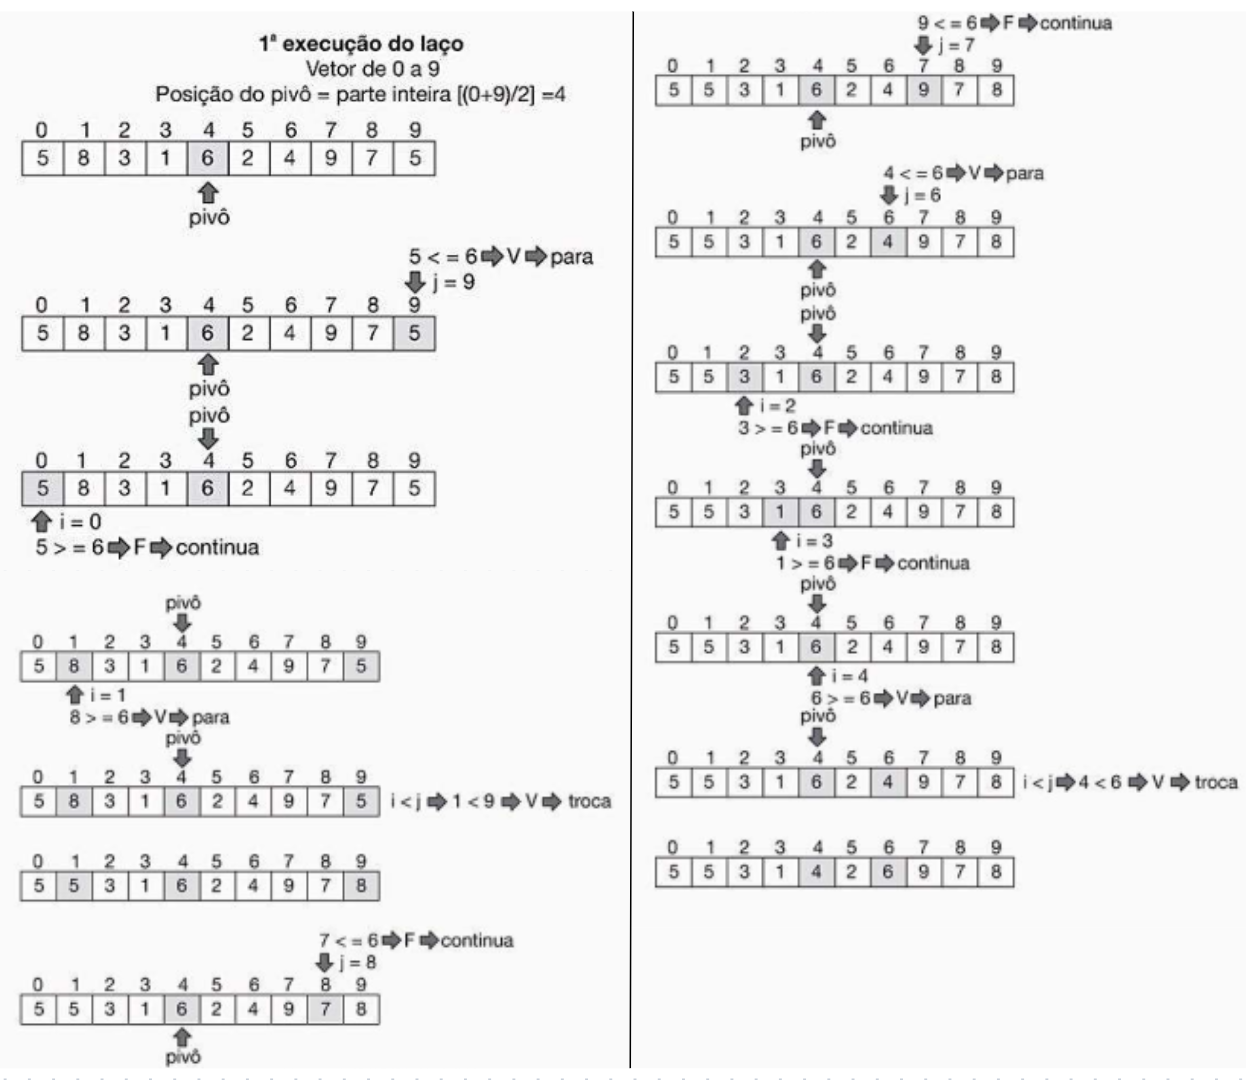
\includegraphics[scale=0.34]{figures/quick/q1.png}
	\caption{Disponível em: ASCÊNCIO, Ana Fernanda Gomes; ARAÚJO, Graziela Santos. Estruturas de Dados: Algoritmos, Análise da Complexidade e Implementações em Java e C/C++.  Pearson; 1ª edição (30 setembro 2015)}
	\label{fig:quick_sort_example}
\end{figure}
\FloatBarrier

\subsection{Quick Sort Recursivo}

Portanto, o caso base da Quick sort recursiva será o intervalo a ser ordenado for tiver 1 elemento ou for vazio. E a etapa recursiva será a chamada da função para a primeira metade até o pivô e segunda metade até o fim da lista.

\begin{algorithm}
	\caption{Quick Sort Recursivo}
	\label{algo:rec_quick_sort}
	\begin{algorithmic}[1]
		\Function{QuickSortRecursivo}{A, limiteEsquerdo, limiteDireito}
		\If{$\text{limiteEsquerdo} \geq \text{limiteDireito}$}
		\Return
		\EndIf
		\State $\text{indicePivot} \gets$ \Call{particao}{$A, \text{limiteEsquerdo}, \text{limiteDireito}$}
		\State \Call{quickSort}{$A, \text{limiteEsquerdo}, \text{indicePivot}$}
		\State \Call{quickSort}{$A, q+1, r$}
		\EndFunction
	\end{algorithmic}
\end{algorithm}
\FloatBarrier

\subsection{Quick Sort Iterativo}

Dado que o Quick Sort é um algoritmo naturalmente recursivo, vamos emular a pilha de execução do computador usando a estrutura de dados pilha, cada chamada recursiva vai ser uma inserção na pilha, e cada etapa de execução será uma remoção na pilha. Com essas considerações, podemos copiar e colar o resto da implementação recursiva.

\begin{algorithm}
	\caption{Iterative Quick Sort}
	\label{algo:iterative_quick_sort}
	\begin{algorithmic}[1]
		\Require{Lista $A$}
		\Ensure{Lista $A$ ordenada}
		\Statex

		\Function{IterativeQuickSort}{$A$}
		\If{$A$ estiver vazio}
		\State \Return
		\EndIf
		\State Crie uma pilha com o par $(0, \text{tamanho de } A - 1)$

		\While{a pilha não estiver vazia}
		\State Remova $(\text{limiteEsquerdo}, \text{limiteDireito})$ do topo da pilha

		\If{$\text{limiteEsquerdo} \geq \text{limiteDireito}$}
		\State \textbf{continue}
		\EndIf
		\State Adicione $(\text{limiteEsquerdo}, \text{indicePivot} - 1)$ na pilha \Comment{Lado esquerdo}
		\State Adicione $(\text{indicePivot} + 1, \text{limiteDireito})$ na pilha \Comment{Lado direito}
		\EndWhile
		\EndFunction
	\end{algorithmic}
\end{algorithm}
\FloatBarrier
\newpage

\subsection{Função auxiliar Partição}

A função partição é responsável pela maior parte do trabalho braçal do Quick Sort, ela é quem organiza uma lista em relação a dterminado pivô

\begin{algorithm}
	\caption{Partição}
	\label{algo:particao}
	\begin{algorithmic}[1]
		\Require{A = $a_1, a_2, a_3, \ldots, a_n$, limiteEsquerdo, limiteDireito}
		\Ensure{O índice do pivô}
		\Function{particao}{$A, \text{limiteEsquerdo}, \text{limiteDireito}$}
		\State pivô $\gets A[\text{limiteDireito}]$
		\State itemEsquerdo $\gets \text{limiteEsquerdo}$
		\For{itemDireito $\gets$ limiteEsquerdo to limiteDireito}
		\If{$A[\text{itemDireito}] <$ pivô}
		\State \textbf{troque} itemDireito por itemDireito em $A$
		\State itemEsquerdo $\gets$ itemEsquerdo $+ 1$
		\EndIf
		\EndFor
		\State \textbf{troque} itemEsquerdo por limiteDireito em A \Comment O pivô é colocado no meio
		\State \Return itemEsquerdo
		\EndFunction
	\end{algorithmic}
\end{algorithm}
\FloatBarrier

\subsection{Análise de Complexidade}

\subsubsection{Análise da versão recursiva}

Primeiro, devemos definir a relação de recorrência do algoritmo.

No procedimento de partição, o tempo de execução é limitado pelo tamanho \( n \) do vetor. Isso ocorre porque ele compara todos os elementos do vetor com o pivô enquanto os índices atenderem a condição \( i < j \). Logo, o procedimento de partição realizará \( O(n) \) comparações.

Os dois vetores gerados pelo procedimento de partição são resolvidos recursivamente. O tamanho desses vetores depende do valor do pivô escolhido na função de partição. Suponha que \( k \) elementos estejam ao lado esquerdo do pivô e \( (n - k - 1) \) elementos estejam à direita do pivô após a partição.

Logo, a complexidade do passo recursivo será a soma das recorrências da ordenação dos dois vetores: \( T(k) + T(n - k - 1) \).

Somando a parte recursiva do algoritmo com o procedimento de partição, teremos:
\[
	T(n) = O(n) + T(k) + T(n - k - 1)
\]

O tempo de execução do Quick Sort depende se o particionamento é ou não balanceado. Se for balanceado, o algoritmo executa tão rapidamente quanto o Merge Sort; caso contrário, ele executará tão lentamente quanto o Insertion Sort. Assim, temos dois casos:

\begin{itemize}
	\item \textbf{Pior caso:} Ocorre quando o pivô é o maior ou o menor elemento do vetor. Aqui, um vetor terá \( n-1 \) elementos e o outro vetor será vazio (não se esqueça do pivô).

	      Para calcular a complexidade do Quick Sort no pior caso, substituímos \( k = n - 1 \) na recorrência encontrada:
	      \[
		      T(n) = O(n) + T(n-1) + T(n - n + 1 - 1)
	      \]
	      \[
		      = cn + T(n-1) \quad \text{(considere \( c \) uma constante)}
	      \]

	      Observe que, neste caso, o algoritmo se comportará da mesma forma que o BubbleSort, que já foi analisado neste trabalho.

	\item \textbf{Melhor caso:} Ocorre quando o pivô é o elemento médio do vetor a ser ordenado em cada chamada do algoritmo de partição. Nessa situação, o processo de partição será balanceado e o tamanho de cada vetor gerado pela partição será, aproximadamente, \( n/2 \).

	      Para calcular a complexidade do Quick Sort nesse caso, substituímos \( k = n/2 \) na recorrência encontrada:
	      \[
		      T(n) = O(n) + T(n/2) + T(n - n/2 - 1)
	      \]
	      \[
		      \approx cn + 2T(n/2)
	      \]

	      Agora, note que o Quick Sort, em seu melhor caso, se comporta da mesma forma do Merge Sort (\ref{sec:merge-sort-teo}), dessa forma sua complexidade no melhor caso é $\Omega(n \cdot \log_2 n)$.

\end{itemize}

\subsubsection{Análise da versão iterativa}

Para determinar a complexidade da versão iterativa, precisamos estimar o tamanho da estrutura de dados "pilha" que simula as chamadas recursivas da outra versão. De forma que seja compreendido quando a estrutura de repetição "while" vai parar. Para tal, teremos dois casos:

\begin{itemize}
	\item \textbf{Melhor caso}: Vamos supor que a função "partição"  sempre particione a lista em duas sublistas iguais, ou seja, o pivô escolhido é sempre a mediana da lista maior, de forma que:
	      \begin{adjustwidth}{-1.8em}{}
		      \begin{tikzcd}[sep=small]
			      &&&& n &&&&& cn \\
			      \\
			      &&& {n/2} && {n/2} &&&& {2 \cdot cn/2 =cn} \\
			      \\
			      & {n/4} && {n/4} && {n/4} && {n/4} && {4 \cdot cn/4 = cn} \\
			      \\
			      {n/8} & {n/8} & {n/8} & {n/8} && {n/8} & {n/8} & {n/8} & {n/8} & {8 \cdot cn/8 = cn} \\
			      \vdots & \vdots & \vdots & \vdots && \vdots & \vdots & \vdots & \vdots \\
			      1 & 1 & 1 & 1 && 1 & 1 & 1 & 1 & {n \cdot c = cn}
			      \arrow[from=1-5, to=3-4]
			      \arrow[from=1-5, to=3-6]
			      \arrow[from=3-4, to=5-2]
			      \arrow[from=3-4, to=5-4]
			      \arrow[from=3-6, to=5-6]
			      \arrow[from=3-6, to=5-8]
			      \arrow[from=5-2, to=7-1]
			      \arrow[from=5-2, to=7-2]
			      \arrow[from=5-4, to=7-3]
			      \arrow[from=5-4, to=7-4]
			      \arrow[from=5-6, to=7-6]
			      \arrow[from=5-6, to=7-7]
			      \arrow[from=5-8, to=7-8]
			      \arrow[from=5-8, to=7-9]
		      \end{tikzcd}
	      \end{adjustwidth}

	      Assim, a recorrência continuará até que \( \frac{n}{2^i} = 1 \), com \( i \) representando o nível da árvore representada acima. Com isso, teremos:

	      \[
		      n = 2^i \implies i = \log_2 n
	      \]

	      Ou seja, a árvore terá \( \log_2 n \) níveis, e cada nível da árvore de recursão realiza um trabalho proporcional a \( n \), devido ao processo de particionamento. Portanto, a complexidade nesse caso será dada por \( T(n) = n \log_2 n \).

	      Assim, podemos dizer que o tempo de execução do algoritmo Quick Sort, em sua forma iterativa no melhor caso, será \( O(n \log n) \), pois:

	      \[
		      \lim_{n \rightarrow \infty} \frac{n \cdot \log_2 n}{n \cdot \log_2 n} =
		      \lim_{n \rightarrow \infty} 1 =
		      1 \in \mathbb{R}^*_+.
	      \]

	      De forma análoga, podemos dizer que este algoritmo será \( \Omega(n \cdot \log_2 n) \) e \( \Theta(n \cdot \log_2 n) \).


	\item \textbf{Pior caso}: Como dito anteiormente, nesse caso, a função partição sempre divide a lista de forma desequilibrada, com o pivô sendo o maior ou o menor elemento do vetor. Nesse cenário, uma das sublistas contém apenas um elemento enquanto a outra contém quase todos os demais. Dessa forma, o particionamento acontece com divisões cada vez menores, resultando em uma árvore de recursão linear, como segue:

	      \[
		      \begin{tikzcd}[sep=small]
			      &&&& n &&&& cn \\
			      &&&& {n - 1} &&&& {c(n - 1)} \\
			      &&&& {n - 2} &&&& {c(n - 2)} \\
			      &&&& \vdots \\
			      &&&& 1 &&&& c
		      \end{tikzcd}
	      \]

	      Neste caso, a altura da árvore de recursão é \( n \), já que em cada nível apenas um elemento é fixado na posição correta, e as sublistas vão sendo reduzidas em apenas um elemento a cada iteração.

	      Assim, o trabalho total realizado por nível é proporcional ao tamanho da lista em cada iteração, somando-se ao longo da altura da árvore. Portanto, a complexidade total é a soma dos primeiros \( n \) números, ou seja:

	      \[
		      T(n) = n + (n - 1) + (n - 2) + \dots + 1 = \frac{n(n + 1)}{2} = \frac{n^2 + n}{2} \approx \frac{n^2}{2}
	      \]

	      Agora, observe que:
	      \[
		      \lim_{n \rightarrow \infty} \frac{\frac{n^2}{2}}{n^2} =
		      \lim_{n \rightarrow \infty} \frac{1}{2} =
		      \frac{1}{2} \in \mathbb{R}^*_+.
	      \]

	      Assim, podemos afirmar que o tempo de execução do Quick Sort, em sua forma iterativa no pior caso, é \( O(n^2) \), \( \Omega(n^2) \) e \( \Theta(n^2) \)


\end{itemize}
